\documentclass[runningheads]{llncs}
\usepackage{graphicx}
\usepackage{amssymb,amsmath}

\begin{document}

\title{Formal Verification for A Buddy Allocation Model Specification
	\thanks{Supported by organization x.}}


\author{Ke Jiang\inst{1} \and
		Yongwang Zhao\inst{2,3} \and
		David San\'{a}n\inst{1} \and
		Yang Liu\inst{1}}

\authorrunning{Ke Jiang et al.}


\institute{School of Computer Science and Engineering, \\
			Nanyang Technological University, Singapore \\ 
	\email{johnjiang,sanan,yangliu@ntu.edu.sg} \and
			School of Computer Science and Engineering, \\
			Beihang University, Beijing, China \and
			Beijing Advanced Innovation Center for Big Data and Brain Computing, \\
			Beihang University, Beijing, China \\
	\email{zhaoyw@buaa.edu.cn}}

\maketitle


\begin{abstract}
Buddy allocation algorithms are widely adopted by memory management systems to manage the address space accessed by applications. However, errors in any stage of the development process of the memory management component, from the specification to the implementation, may lead to critical issues in other components using it. We apply formal methods to ensure the absence of any misbehavior. Rigorous mathematical proofs provide strong assurance to the development process. In this paper, we firstly present a specification for the buddy allocation algorithm. And thence we validate enough properties to guarantee functional correctness of this algorithm. Finally, we construct execution traces to verify the integrity for security. Through these efforts, we propose a buddy allocation model that provides both functional correctness and security. Also, we use interactive theorem prover Isabelle/HOL to carry out the verification work.

\keywords{Memory Specification \and
		Formal Verification \and
		Functional Correctness \and
		Security.}
\end{abstract}


\section{Introduction}
In the past several decades, buddy allocation algorithms have been applied in the memory management systems. Errors in any stage of the development process of the memory management component may lead to critical issues in other components who invoke it. To improve confidence on the reliability of the development process, verification of functional correctness and security properties is applied into each stage, from the specification level to the implementation level, even the machine code level. Formal methods have been successfully applied in the verification of many critical systems due to these methods provide strong assurance by rigorous mathematical proofs. Therefore, we apply formal methods to ensure the absence of any misbehavior during the development process of the buddy allocation model.

here is related work.

In this paper, we propose a buddy allocation model, which supports both functional correctness and security. To achieve this goal, we develop a specification for buddy allocation algorithms by functional programming in Isabelle/HOL proof assistant. Our specification must consists of algorithm details as specific as possible for the sake of capturing any feature in the algorithms. Then we design a series of properties for functional correctness of the algorithm. After that, we apply theorem-proving method to prove these properties. To verify integrity for security, we construct execution traces based on event, and then prove that the operation of one domain on memory does not affect any other domains. So far, we have completed the construction and verification of the buddy allocation algorithm.

The following section briefly introduces the Isabelle/HOL verification environment. The next section is about the formalization of buddy allocation model including representation of our specification and proofs to properties for functional correctness. The verification of integrity for security is arranged in the following section. The last section is about the conclusions and future work.


\section{Isabelle/HOL Verification Environment}
Our specification and verification work is based on the interactive theorem prover Isabella/HOL. HOL represents the Higher-Order Logical and Isabelle is its generic interactive theorem prover. In Isabelle/HOL, it is usual to employ functional programming method to define a function and to adopt theorem proving technique to reason a lemma or a theorem. For a gentle introduction to Isabelle/HOL see~\cite{reg_Isabelle/HOL}. 

Apart from commonly used types like \textsl{bool} and \textsl{nat}, Isabelle offers notion \textsl{datatype} to create a distinguished element to some existing types. Projection functions \textsl{fst} and \textsl{snd} comes with the tuple (\textsl{$t_1$} $\times$ \textsl{$t_2$}). Notions \textsl{list} and \textsl{set} are used as constructors to create a collection of same type. Operation 'cons' denoted by '$\#$' on a list means that adding an element to the head of list. The \textsl{i}th component of a list \textsl{xs} is written as \textsl{xs}!\textsl{i}. \textsl{SOME x} and \textsl{THE x} in the \textsl{set A} represent choosing an element arbitrarily, existing and unique element respectively. Furthermore, $\lambda$-abstractions are also contained in terms like $\lambda$(\textsl{x, y}). \textsl{f x y}.

Non-recursive definition can be made with the \textbf{definition} command and the \textbf{primrec} function definition is used for primitive recursions. The notation $\lbrack$ $A_1$;\dots;$A_n$$\rbrack$ $\Longrightarrow$ A represents an implication with assumptions $A_1$;\dots;$A_n$ and conclusion A. Isabelle mainly employs backward deduction, which means to prove the main goal, we must firstly prove subgoals which are decomposed from the main goal. It uses the rules of the reasoning like introduction, elimination, destruction rules, etc., as well as automatic provers such as \textsl{SMT}.


\section{Formalization of Buddy Allocation Model}
The formalization of buddy allocation models consists of a specification for algorithms and proofs to properties for functional correctness. The challenge is that we apply quartering from Zephyr OS for buddy allocation operations, which brings complexity to proofs.

\subsection{Memory Model Specification}
The specification begins with the fundamental structure of a quad-tree.
\begin{align*}
(set:\ 'a)\ tree = &Leaf\ (L:\ 'a)\ | \\
&Node\ (LL:\ 'a\ tree)\ (LR:\ 'a\ tree)\ (RL:\ 'a\ tree)\ (RR:\ 'a\ tree) \\
&for\ map: tree\_map
\end{align*}
The quad-tree constructed by induction contains two pieces of information: the memory block state (indicated as \textsl{ALLOC} and \textsl{FREE} respectively); a address tag occupied by a memory block (indicated as \textsl{ID}). The mapping function \textbf{set} assists to collect the leaves from a tree. With the help of the block state and the function \textbf{get\_level}, allocated leaves or free leaves from different levels can be gathered by \textbf{allocsets}, \textbf{freesets} and \textbf{freesets\_level}. To create a new leaf, we have to pick up a new \textsl{ID} to this new leaf by the strategy of \textsl{SOME p. p} $\notin$ \textsl{idset}. Later, we will prove that with this strategy, all leaves have different \textsl{IDs}.

Based on the above quad-tree structure, next we specify two operations with the buddy algorithms: \textbf{alloc} and \textbf{free}. For \textsl{rsize} (the size of requested memory block) in allocation operation, there is a definition that maps it to the level of the quad-tree and gives the most suitable level \textsl{rlv}. The concept of \textsl{most suitable level} will be proved in the next subsection. For the specification, we only use level for both the memory blocks of the quad-tree and requested memory block. And the smaller the level, the larger size the memory block.

\begin{definition} {exists\_freelevel} \\
exists\_freelevel blo\_set lv $\equiv$ $\exists$l. l $\leq$ lv $\wedge$ $\exists$b $\in$ blo\_set. freesets\_level b l $\ne$ $\emptyset$
\end{definition}

\begin{definition} {freesets\_maxlevel}\\
freesets\_maxlevel blo\_set lv $\equiv$ \\
\phantom{x} \hspace{10pt} THE lmax. lmax $\leq$ lv $\wedge$ \\
\phantom{x} \hspace{60pt} $\exists$b $\in$ blo\_set. freesets\_level b lmax $\neq$ $\emptyset$ $\wedge$ \\
\phantom{x} \hspace{60pt} $\forall$l $\leq$ lv. $\exists$b $\in$ blo\_set. freesets\_level b l $\ne$ $\emptyset$ $\longrightarrow$ l $\leq$ lmax
\end{definition}

\begin{definition} {Allocation Operation} \\
alloc blo\_set rlv $\equiv$ \\
\phantom{x} \hspace{10pt} if exists\_freelevel blo\_set rlv then \\
\phantom{x} \hspace{20pt} lmax = freesets\_maxlevel blo\_set rlv \\
\phantom{x} \hspace{20pt} if lmax = rlv then \\
\phantom{x} \hspace{30pt} btree = SOME b. b $\in$ blo\_set $\wedge$ freesets\_level b rlv $\ne$ $\emptyset$ \\
\phantom{x} \hspace{30pt} l = SOME l. l $\in$ freesets\_level btree rlv \\
\phantom{x} \hspace{20pt} else \\
\phantom{x} \hspace{30pt} btree = SOME b. b $\in$ blo\_set $\wedge$ freesets\_level b lmax $\ne$ $\emptyset$ \\
\phantom{x} \hspace{30pt} l = split (SOME l. l $\in$ freesets\_level btree lmax) (rlv - lmax) \\
\phantom{x} \hspace{10pt} else False
\end{definition}

The first step of allocation is to check whether there is a quad-tree in \textsl{blo\_set} (the memory pool tree collection), that has such free memory blocks whose level is less than or equal to \textsl{rlv}. This step is done by \textbf{exists\_freelevel}, and if it returns \textsl{False} then the allocation progress stops. Otherwise, the next step conducted by \textbf{freesets\_maxlevel} is to return the maximum level among all levels with free memory blocks. If the maximum level is equal to \textsl{rlv}, then any free memory block in \textsl{rlv} is to be allocated. If not, any free memory block in the maximum level is to be conducted by \textbf{split} showed in Fig. \ref{fig1} until free memory block in \textsl{rlv} appears and then be allocated. The state of the assigned leaf is set to \textsl{ALLOC}.

\begin{figure}
\centering
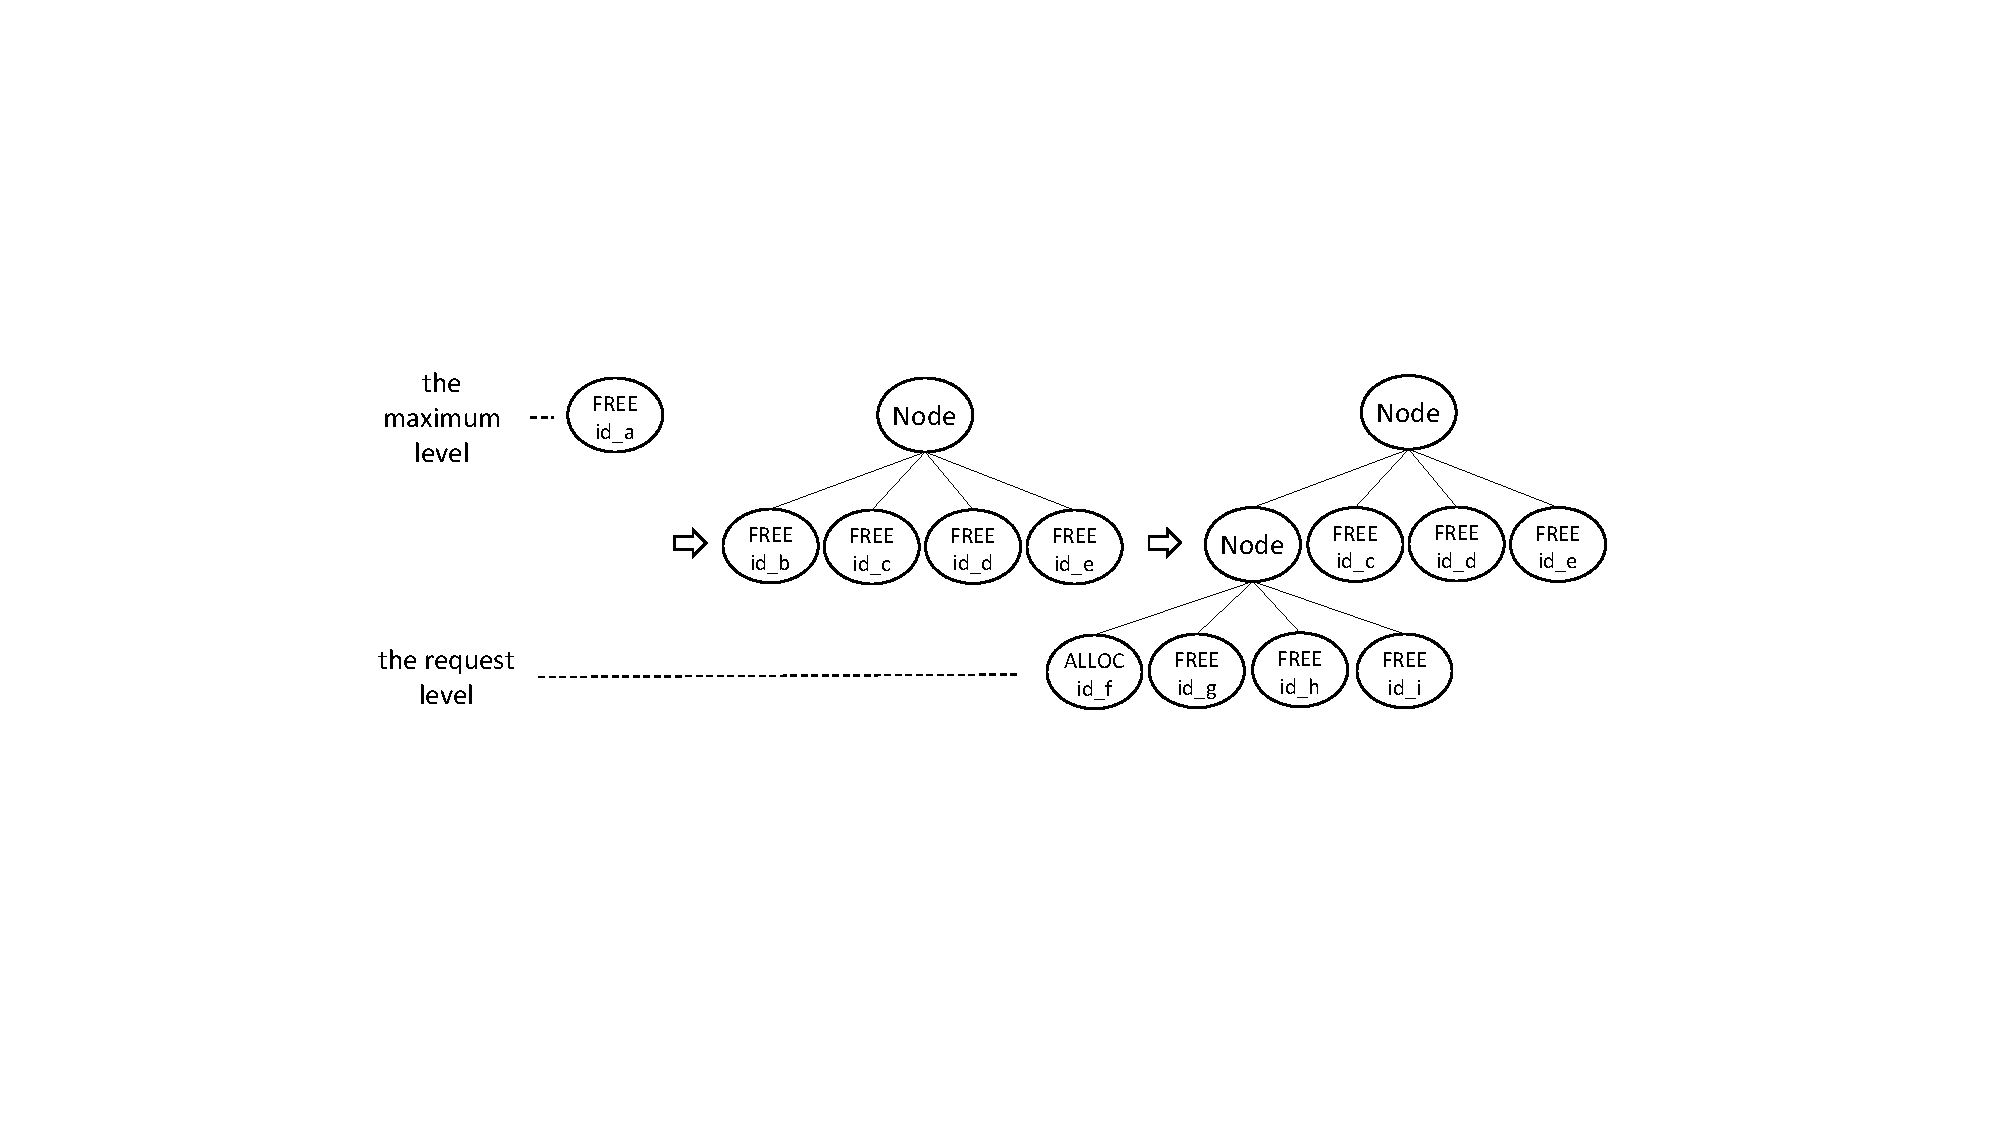
\includegraphics[width=1\textwidth]{fig1.pdf}
\caption{The progress of dividing a free memory block}
\label{fig1}
\end{figure}

\begin{definition} {Deallocation Operation} \\
free blo\_set b $\equiv$ \\
\phantom{x} \hspace{10pt} if $\exists$btree $\in$ blo\_set. b $\in$ tree.set btree then \\
\phantom{x} \hspace{20pt} if State b = FREE then False \\
\phantom{x} \hspace{20pt} else btree = THE t. t $\in$ blo\_set $\wedge$ b $\in$ tree.set t \\
\phantom{x} \hspace{40pt} merge (reset btree b FREE) \\
\phantom{x} \hspace{10pt} else False
\end{definition}

The deallocation progress firstly checks whether there is a quad-tree in \textsl{blo\_set} that the occupied memory block to be released belongs to this tree. If there is no such tree, the procedure returns \textsl{False}. Next, if the state of the occupied memory block is \textsl{FREE}, the progress also returns \textsl{False}. When all conditions are met, the memory block is returned to the tree it belongs to, thereafter merging operation is executed. The merging operation is to combine all free memory blocks that belong to the same parent tree showed in Fig. \ref{fig2}.

\begin{figure}
\centering
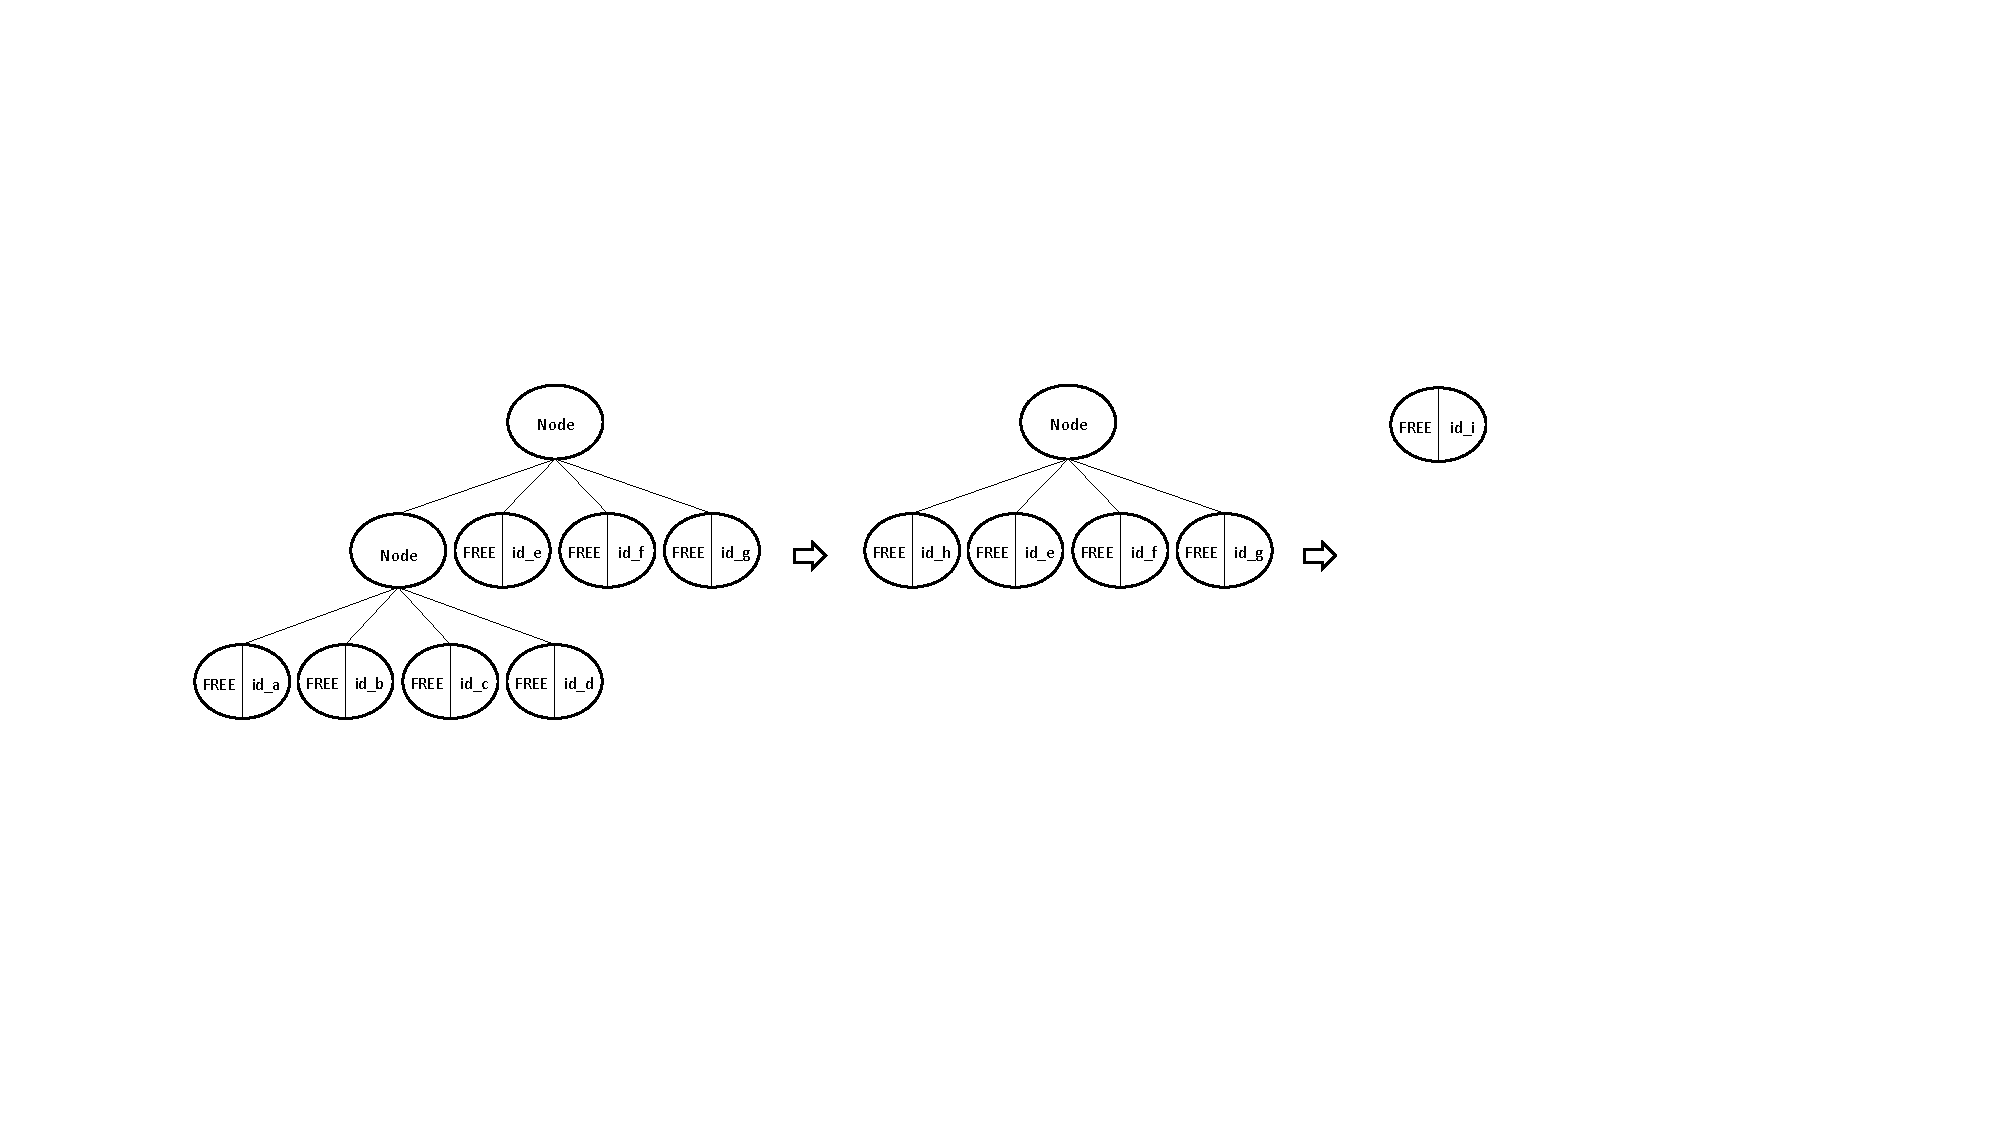
\includegraphics[width=1\textwidth]{fig2.pdf}
\caption{The progress of merging all free memory blocks}
\label{fig2}
\end{figure}

At this point, we have done the specification for the buddy memory algorithm. Next, we are going to verify some properties to guarantee the functional correctness of this specification.


\subsection{Memory Model Properties}
Once the specification is finished, the preconditions $\&$ postconditions for functions as well as the invariants are to be raised up to ensure the functional correctness of the specification. We try to answer these questions: Dose the algorithm pick out the most suitable block from all the available blocks? Does the algorithm correctly adjust the state of the relevant memory block after allocation and deallocation? How the algorithm make sure to execute the merging operation after deallocation? How the specification ensure the correctness of the quad-tree structure? What invariants does the specification preserve? Dose the algorithm satisfy some security properties? Answering these questions contributes to the construction of a reliability system. We give preconditions and postconditions in the first place.

\begin{definition} {Preconditions $\&$ Postconditions} \\
When call allocation, if \textbf{exists\_freelevel} returns false, then allocation fails; \\
When call allocation, if \textbf{exists\_freelevel} returns true and \textbf{freesets\_maxlevel} returns exactly the level to be allocated, then directly allocate; \\
When call allocation, if \textbf{exists\_freelevel} returns true and \textbf{freesets\_maxlevel} returns not the level to be allocated, then allocate through splitting; \\
When call releasing, if the memory block to be freed dose not belong to this memory pool, then releasing fails; \\
When call releasing, if the memory block to be free belongs to this memory pool, then free the block and merge; \\
When allocation fails, if the thread will wait, then suspend this thread, insert it to the pool's waiting queue and schedule; \\
When releasing succeeds, if the pool's waiting queue is not empty, then wake all suspended threads.
\end{definition}

\begin{theorem}
The buddy memory model satisfies the preconditions and postconditions.
\end{theorem}

These conditions are very simple because of the functional construction of the model. They are also very easy to understand and do not require additional explanation. These conditions only ensure that the buddy model follows the design idea of the algorithm on the execution branches. However, they do not involve the design details inside the model. In other words, we need more invariants to ensure that the internal details of the model follow the design idea of the algorithm.

To make sure that we execute \textbf{alloc} and \textbf{free} on the right level of quad tree, we have to specify that the level of root is zero and the level of below leaf is one more level than the upper leaf. Thus, we introduce the following lemma.

\begin{lemma}
	The level of root is zero and the level of below leaf is one more level than the upper leaf.
\end{lemma}

Then the question is that whether we choose a most suitable memory block for allocation. As we mentioned earlier, there is a mapping between the quad-tree hierarchy and the size of memory block. If we use static linked list \textsl{blo\_list} to store block size at each level, we have the following mapping definition:

\begin{definition} {Mapping Sizes $\&$ Levels} \\
output\_level = THE l. l $<$ length blo\_list $\wedge$ request\_size $\le$ blo\_list ! l $\wedge$ (length blo\_list $>$ 1 $\wedge$ l $<$ length blo\_list - 1) $\longrightarrow$ request\_size $>$ length blo\_list ! (l+1)
\end{definition}

We use \textsl{blo\_list} of listing structure to record the mapping relation between request block size and quad tree's level. Due to the listing structure, quad tree's level can be expressed by the index of this list. Definition 2 gives us a function that how to get a suitable layer to allocate with the \textsl{blo\_list}. A suitable layer means that the block size it represents has to be greater than or equal to the request block size, and there is no layer below it that meets the size condition. We indicate that any request block size which is greater than the first layer's size is not allowed because we handle this condition as an exception.

\begin{theorem}
Any request block whose size is smaller than or equal to the first layer's size can be mapped to such a suitable quad tree level.
\end{theorem}

Now, with lemma 1 and theorem 2, we can make sure that any operation on block size can be executed correctly on the right level of quad tree.

Another question in the memory allocation algorithm is the fragmentation. Many reasons are responsible to this phenomenon. In this case, definition 2 which maps block size to relevant quad tree level and the \textsl{blo\_list} eliminate internal fragmentation. We believe that external fragmentation in buddy memory allocation algorithm is caused by the fact that all free leaves from the same level and belong to the same root tree are not merged into the upper leaf after the release operation. According to the algorithm, this situation should not be allowed. Thus, we design the following theorem to ensure the external fragmentation in-existence.

\begin{theorem}
There is not existence of such circumstance that all leaves from the same level and belong to the same root tree are FREE.
\end{theorem}

This theorem is relative to a sub-operation in \textbf{free}, merge operation. Merge operation is important to handling the external fragmentation. The core service in the merge operation is to check whether the memory block to be released with all other leaves forms the situation that all leaves from the same level and belong to the same root are \textsl{FREE}. If this happens, then merge operation has to combine these leaves into an upper leaf. The merge operation is a inductive progress until there is not existence of such nodes and leaves. Theorem 3 guarantees that merge operation has been done at every time and got the correct result.

According to the facts that: (1)the status of a running thread is \textsl{RUNNING}; (2)the status of any thread in waiting queue is \textsl{BLOCKED}. This theorem guarantees the correctness of a thread's status before and after each operation. The theorem is as follows.

\begin{theorem}
(\textsl{current\_thread} $\neq$ \textsl{nil} $\longrightarrow$ \textsl{Status} (\textsl{current\_thread}) = \textsl{RUNNING}) $\wedge$ (\textsl{waiting\_queue} $\neq$ $\lbrace$$\rbrace$ $\wedge$ \textsl{t} $\in$ \textsl{waiting\_queue} $\longrightarrow$ \textsl{Status} (\textsl{t}) = \textsl{BLOCKED})
\end{theorem}

Above the \textsl{alloc}, \textsl{free} and \textsl{schedule} operations layer, we add the concept of thread to simulate the real situation of the whole memory management system. No matter which operation a thread invokes and what the results it gets, the only thing we need to make sure is that the thread state is correct. Thus theorem 4 guarantees this very well.

In the end, we turn to two significant properties: isolation and non-leakage. Memory isolation means that any two blocks of memory will not overlap at the address. In the event of an overlap in the address, incorrect information will directly cause confusion and errors in the program, as well as serious consequences. Memory leakage means that available memory blocks (including allocated memory blocks and unallocated memory blocks) are getting less and less. In the case of program security, some malicious programs modify the size of available memory to achieve the purpose of attacking.

Before revealing this two properties, we introduce a concept of \textsl{ID} to represent the address range of a memory block and a lemma to maintain the relation between \textsl{ID} and address range.

\begin{definition} {Mapping IDs $\&$ Addresses} \\
The root tree addresses from root\_address\_start to root\_address\_end, the leaf $\alpha$ with ID is one of child leaves of root tree whose index is leaf\_index. \\
Then there is a mapping that ID represents the following range of address: \\
$\alpha$\_address\_start = root\_address\_start + leaf\_index $\times$ $\frac{Size (root\_tree)}{n}$ \\
$\alpha$\_address\_end = $\alpha$\_address\_start + $\frac{Size (root\_tree)}{n}$
\end{definition}

With this definition, we have to guarantee the one-to-one mapping relation between the \textsl{ID} and the range of addresses. Then we have the following lemma to ensure this.

\begin{lemma}
For any range of addresses in the memory pools, there is uniquely one ID of leaf in some Block tree corresponding to it.
\end{lemma}

Then we adopted a series of strategies to produce such an \textsl{ID}. There is no overlap in memory addresses, which translates to all \textsl{ID}s being different.

\begin{theorem}
If Block tree $\alpha$ is such a tree whose all IDs of leaves are different, then after any operations, the new tree maintains this property.
\end{theorem}

With lemma 2 and theorem 5, we can say that all ranges of memory addresses are isolated and there is no overlap between them.

Due to we use the structure of tree and we have mapped all the memory blocks into the leaves in these tree, it becomes easy to prove the non-leakage of memory. In a tree, we have this understanding: all the leaves including allocated and unallocated leaves are all in use. Thus once we prove the number relationship between the nodes and the leaves of the N-tree, we can say that all the leaves are in use and none leaf is forgotten.

\begin{lemma}
N-tree: Num (Leaf) = Num (Node) $\times$ n + 1
\end{lemma}

\begin{theorem}
If Block tree $\beta$ is such a tree whose number of leaf and node has above relation, then after any operations, the new tree maintains this property.
\end{theorem}

With lemma 3 and theorem 6, we can ensure that all memory blocks are in use and none of them is forgotten or stolen.

To sum up, in this section we introduce the N-tree structure to simulate memory because of the buddy operation methods. Then we give a specification of the algorithm including \textbf{alloc}, \textbf{free} and \textbf{schedule}. After that, we give axiomatic proof for functional correctness including preconditions and postconditions, the most suitable allocated size, invariants during execution, memory isolation and non-leakage. Through these specifications and proof, we guarantee to give a functionally correct buddy memory model, which is significant to the next security model.


\section{Model Memory Security}
The concept of noninterference is introduced in~\cite{reg_noninterference} to provide a formalism for the specification fo security policies. The main idea is that domain \textsl{u} is non-interfering with domain \textsl{v} if no action performed by \textsl{u} can influence the subsequence outputs seen by \textsl{v}.

\subsection{Memory Execution Model}
Considering the fact that the execution of the buddy memory allocation is expressed as a series of operating actions among initialization, allocation, release, scheduler and time-ticking in a serial system, we introduce an event framework to simulate the whole processing of the entire system. Another factor of introducing this framework is that we can verify whether the states before and after an execution both satisfy a certain property of correctness or security.

As we define, \textsl{State} is the basic element of the execution trace. The execution of each operation must follow a certain order, therefore the trace is defined as a \textsl{list} of type \textsl{State}. A trace is defined looks like this:

\phantom{x} \textbf{type\_synonym} \textsl{Trace} = "\textsl{State list}" \\

Different orders of execution of operations compose different execution pathways. For modeling all the possible pathways, we introduces a collection for all execution pathways in a inductive way.

\phantom{x} \textbf{inductive\_set} \textsl{execution} :: "\textsl{Trace set}" \textsl{where} \\
\phantom{x} \hspace{3pt} \textsl{zero\_exe}: "$\lbrack$\textsl{s}$\rbrack$ $\in$ \textsl{execution}" $\mid$ \\
\phantom{x} \hspace{3pt} \textsl{init\_exe}: "$\lbrack$\textsl{es} $\in$ \textsl{execution}; \textsl{fst} (\textsl{k\_mem\_pool\_define s nam nlv num}) = \textsl{t}; \textsl{t} = \textsl{es} ! \textsl{0}$\rbrack$ $\Longrightarrow$ \textsl{s} \# \textsl{es} $\in$ \textsl{execution}" $\mid$ \\
\phantom{x} \hspace{3pt} \textsl{alloc\_exe}: "$\lbrack$\textsl{es} $\in$ \textsl{execution}; \textsl{po} $\in$ \textsl{set} (\textsl{pools s}); \textsl{fst} (\textsl{k\_mem\_pool\_alloc s po lv ti}) = \textsl{t}; \textsl{t} = \textsl{es} ! \textsl{0}$\rbrack$ $\Longrightarrow$ \textsl{s} \# \textsl{es} $\in$ \textsl{execution}" $\mid$ \\
\phantom{x} \hspace{3pt} \textsl{free\_exe}: "$\lbrack$\textsl{es} $\in$ \textsl{execution}; \textsl{po} $\in$ \textsl{set} (\textsl{pools s}); \textsl{fst} (\textsl{k\_mem\_pool\_free s po num}) = \textsl{t}; \textsl{t} = \textsl{es} ! \textsl{0}$\rbrack$ $\Longrightarrow$ \textsl{s} \# \textsl{es} $\in$ \textsl{execution}" $\mid$ \\
\phantom{x} \hspace{3pt} \textsl{tick\_exe}: "$\lbrack$\textsl{es} $\in$ \textsl{execution}; \textsl{time\_tick s} = \textsl{t}; \textsl{t} = \textsl{es} ! \textsl{0}$\rbrack$ $\Longrightarrow$ \textsl{s} \# \textsl{es} $\in$ \textsl{execution}" $\mid$ \\
\phantom{x} \hspace{3pt} \textsl{schedule\_exe}: "$\lbrack$\textsl{es} $\in$ \textsl{execution}; \textsl{schedule s} = \textsl{t}; \textsl{t} = \textsl{es} ! \textsl{0}$\rbrack$ $\Longrightarrow$ \textsl{s} \# \textsl{es} $\in$ \textsl{execution}" \\

Firstly, the trace list which has only one state belongs to the execution pathways. Secondly, five operations on trace list have same pattern. Taking initialization function as an example. The \textsl{es} is one execution pathway of type \textsl{list} and initialization function translates the previous state \textsl{s} into state \textsl{t}. If the state \textsl{t} is the first element of list \textsl{es}, then we can add state \textsl{s} to the head of execution pathway \textsl{ex} to form a new list (\textsl{s} \# \textsl{es}). Eventually, the new list (\textsl{s} \# \textsl{es}) is also one execution pathway.

Thereafter, we have to define a reachable set using the execution trace. The purpose of introducing reachable set whose execution trace starts from \textsl{s0} is to prove all properties are established on reachable set. Following is the definition of reachable set.

\phantom{x} \textbf{definition} "\textsl{reachable s t} $\equiv$ ($\exists$\textsl{s} $\in$ \textsl{execution}. \textsl{ts} ! \textsl{0} = \textsl{s} $\wedge$ \textsl{last ts} = \textsl{t})" \\
\phantom{x} \hspace{3pt} \textbf{definition} "\textsl{reachable0 s} $\equiv$ \textsl{reachable s0 s}" \\
\phantom{x} \hspace{3pt} \textbf{definition} "\textsl{ReachStates} $\equiv$ $\lbrace$\textsl{s}. \textsl{reachable0 s}$\rbrace$"

But how to connect the allocation operation and releasing operation? The answer is the scheduling. According to the C-code level in Zepyhr OS, two places need the participation of scheduling: (1).Once the memory allocation process fails and one of the thread's parameters indicates that it will wait, we need to add the thread to the corresponding memory pool's waiting queue and then schedule another thread to run. (2).Each time after the releasing operation, the algorithm checks if there are any threads in the waiting queue of the memory pool. If there are, it wakes up all threads and scheduler arranges for one thread to execute. Although scheduling operation is not the primary role in memory algorithm verification, for algorithmic integrity, we introduce an abstract scheduling which takes any thread from the ready queue to our buddy memory model.


\subsection{Security Proofs}


\section{Conclusions and Future Work}
To sum up, we give a specification for buddy memory allocation algorithm. 

\begin{thebibliography}{8}
\bibitem{reg_Isabelle/HOL}
T. Nipkow, L. C. Paulson, and M. Wenzel. Isabelle/HOL-A Proof Assistant for Higher-Order Logical, volume 2283 of LNCS. Springer-Verlag, 2002.

\bibitem{reg_noninterference}
J. Goguen and J. Meseguer. Security Policies and Security Models, Proceedings of the IEEE Computer Society Symposium on Research in Security and Privacy, 1982, p. 11-20.


\end{thebibliography}


\end{document}